\documentclass[a4paper,11pt]{article}

% --- Encodage et langue
\usepackage[utf8]{inputenc}     % accents directement dans le source
\usepackage[T1]{fontenc}        % césure correcte des mots accentués
\usepackage[french]{babel}      % typographie française
\usepackage{newtxtext,newtxmath} % police Times moderne, rendu « journal »

% --- Mise en page
\usepackage[margin=2.5cm]{geometry}
\usepackage{microtype}
\usepackage{fancyhdr}
\pagestyle{fancy}
\fancyhead[L]{\small\itshape Détection des véhicules de petite taille
              en trafic urbain dense}
\fancyhead[R]{\small\thepage}
\fancyfoot[C]{}
\renewcommand{\headrulewidth}{0.4pt}

% --- Sciences
\usepackage{amsmath}  % amssymb inutile : newtxmath fournit les symboles AMS
\usepackage{siunitx}
\sisetup{locale = FR}           % \num{0.438} s'affiche « 0,438 »
\usepackage{graphicx}
\usepackage{booktabs}
\usepackage[font=small,labelfont=bf]{caption}
\usepackage{subcaption}
\usepackage{xcolor}

% --- Couleurs du projet (celles de l'application de démonstration)
\definecolor{bleunuit}{HTML}{0F3460}
\definecolor{terrecuite}{HTML}{C1502E}

% --- Graphiques
\usepackage{pgfplots}
\pgfplotsset{compat=1.18}
\usetikzlibrary{positioning, arrows.meta}

% --- Liens et références (hyperref en dernier ou presque)
\usepackage[colorlinks=true, linkcolor=bleunuit, citecolor=bleunuit,
            urlcolor=terrecuite]{hyperref}
\usepackage[french,nameinlink]{cleveref}
\usepackage{qrcode}             % QR code vers la démonstration en ligne

% --- Marqueur des éléments manquants : à faire disparaître avant le rendu
\newcommand{\todo}[1]{\textcolor{red}{\textbf{[À FAIRE : #1]}}}

\begin{document}

% ============================ Page de garde ============================
\begin{titlepage}
  \centering

  {\scshape Académie des Mathématiques Appliquées (Bénin)\par}
  \vspace{2pt}
  {\small Programme d'Introduction à l'IA · Cohorte 2\par}
  \vspace{10pt}
  {\color{terrecuite}\rule{\linewidth}{0.8pt}}

  \vfill

  {\LARGE\bfseries Détection des véhicules éloignés, de petite taille\\
   et dans les embouteillages\par}
  \vspace{14pt}
  {\color{terrecuite}\rule{5em}{2.5pt}}
  \vspace{14pt}

  {\large Scène de trafic urbain appliquée au contexte béninois :\\
   proposition d'amélioration basée sur YOLOv8\par}

  \vfill

  \begin{minipage}{0.48\linewidth}
    \centering
    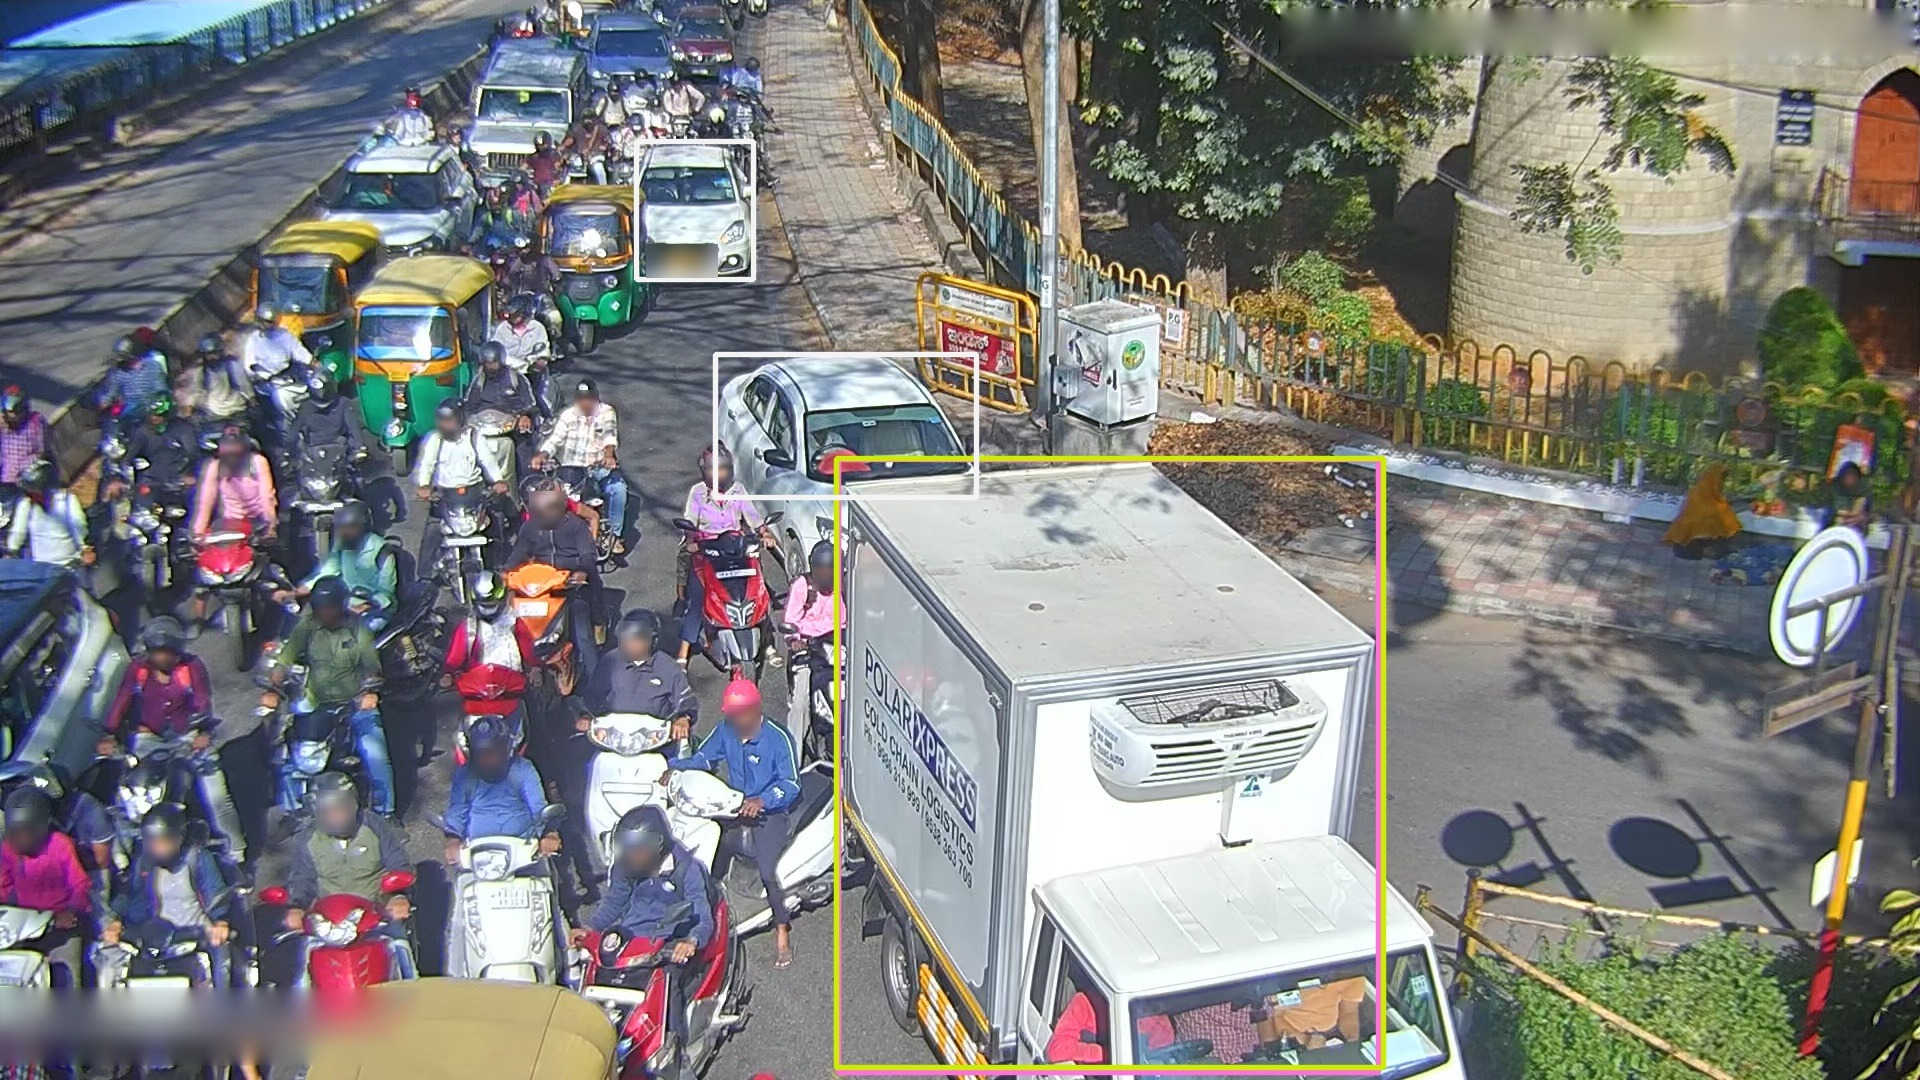
\includegraphics[width=\linewidth]{figures/scene1_base.jpg}\\[4pt]
    {\footnotesize\color{bleunuit}\bfseries AVANT\hspace{0.5em}}%
    {\footnotesize 4 véhicules détectés}
  \end{minipage}
  \hfill
  \begin{minipage}{0.48\linewidth}
    \centering
    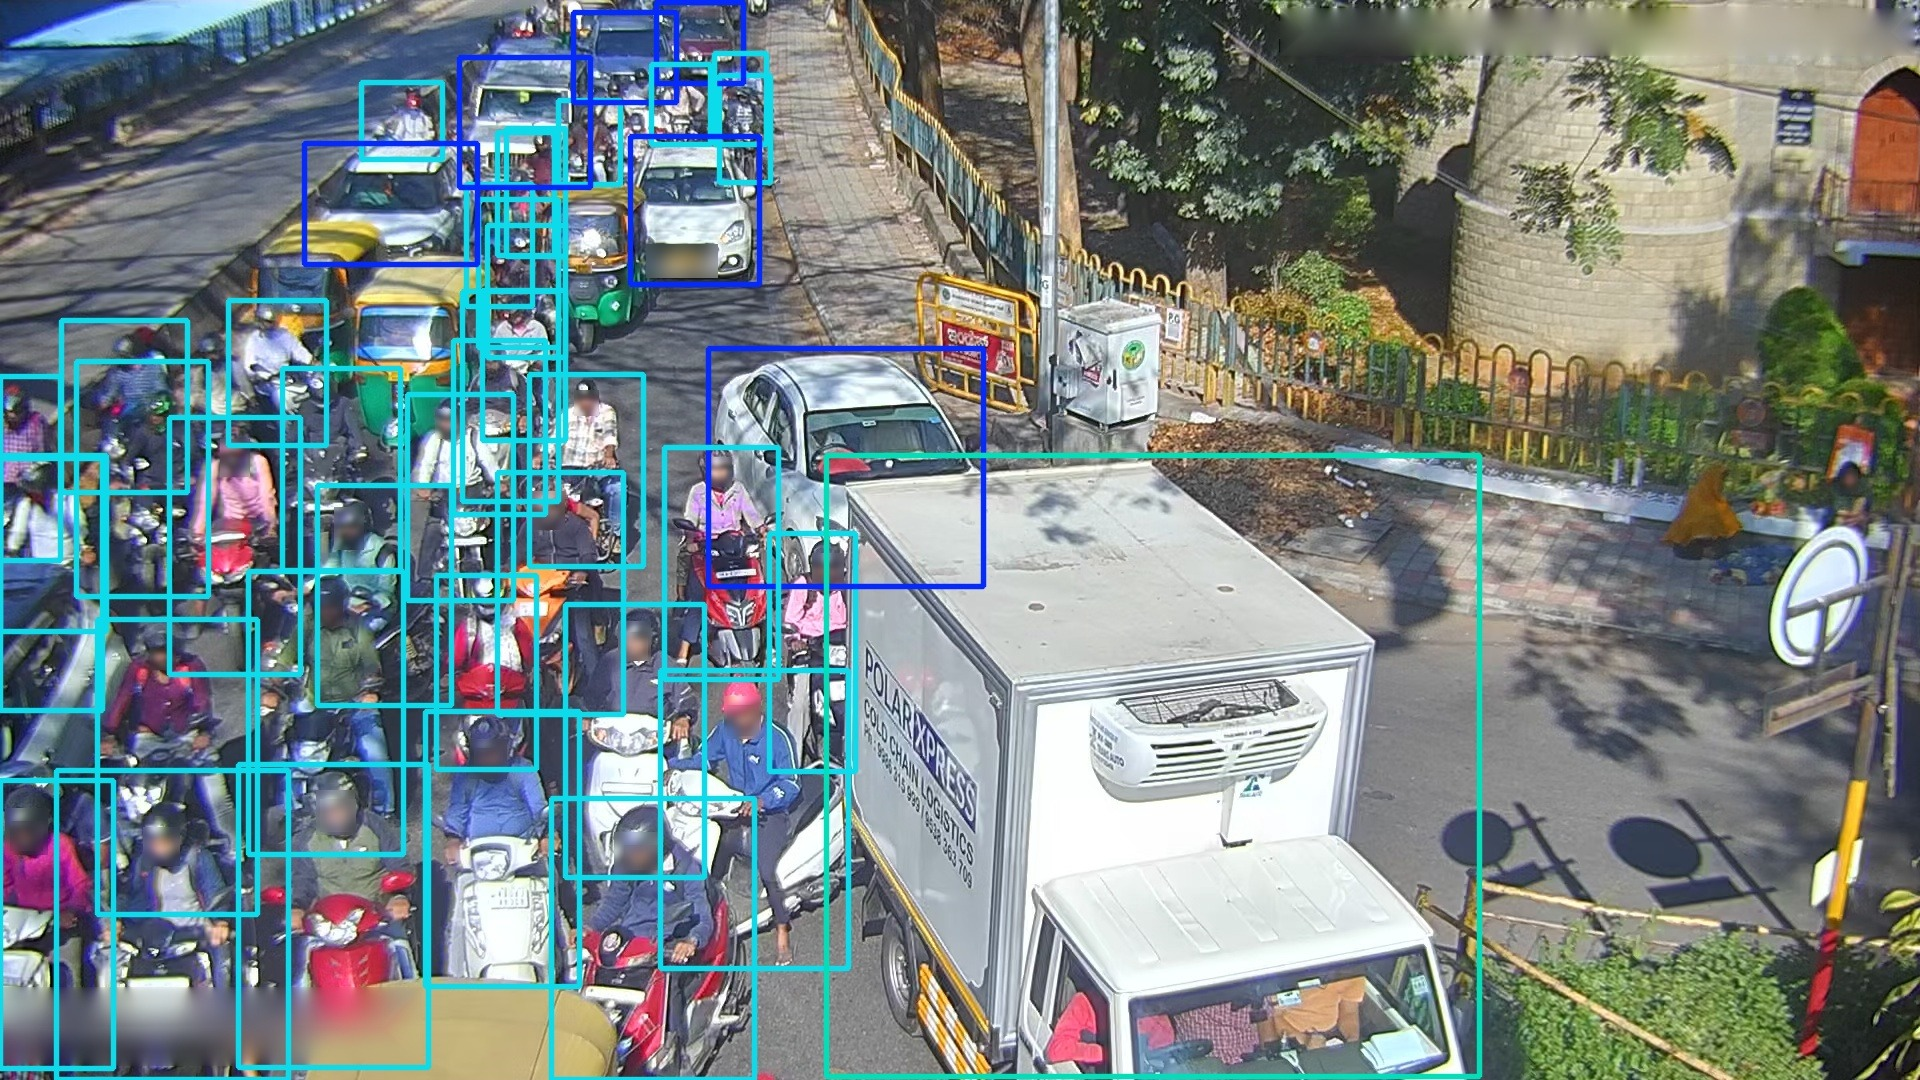
\includegraphics[width=\linewidth]{figures/scene1_finetune.jpg}\\[4pt]
    {\footnotesize\color{terrecuite}\bfseries APRÈS\hspace{0.5em}}%
    {\footnotesize 44 véhicules détectés}
  \end{minipage}

  \vspace{6pt}
  {\scriptsize\color{gray} Même scène du jeu de test, avant et après
   fine-tuning (image \texttt{val\_000556}).\par}

  \vfill

  {\large Aïchatou Traoré · Benoît Djossou · Andréa Afouda\par}
  \vspace{6pt}
  {\small Projet Intégrateur 1 · Groupe 5\par}
  \vspace{14pt}
  {\color{terrecuite}\rule{\linewidth}{0.8pt}}
  \vspace{8pt}

  {\small Août 2026\hspace{2em}·\hspace{2em}Démonstration en ligne :
   \url{https://detection-vehicules-benin.streamlit.app}\par}

\end{titlepage}
% =======================================================================

\begin{abstract}
La République du Bénin a engagé la mise en place d'un système national
de vidéoprotection dont la vidéo-verbalisation par vision par ordinateur
est une application clef. Le premier maillon du pipeline, la détection
des véhicules, échoue le plus souvent sur les véhicules éloignés, de
petite taille à l'image ou masqués dans les embouteillages, qui sont
précisément les configurations dominantes du trafic urbain
ouest-africain. Nous
étudions si un fine-tuning de YOLOv8n sur du trafic urbain dense
améliore cette détection. Faute de jeu de données béninois public, nous
utilisons un sous-ensemble reproductible de 3\,000 images
(25\,688 véhicules annotés) de BMD-45, jeu de caméras CCTV de Bengaluru
structurellement comparable (caméras fixes, forte densité, $56\,\%$ de
deux-roues), remappé vers quatre classes alignées sur COCO. Le protocole
de comparaison garantit l'équité entre modèle pré-entraîné et modèle
fine-tuné : mêmes images et boîtes de test, réindexation des classes,
rappel ventilé par taille d'objet selon la convention COCO avec aires
normalisées à la résolution d'entrée du réseau. Après 50 epochs, la
mAP@0,5 passe de $0{,}438$ à $0{,}825$ ($+88{,}4\,\%$) et le rappel des
objets de moins de $32 \times 32$ pixels de $0{,}122$ à $0{,}694$
($+469{,}4\,\%$), le gain étant d'autant plus fort que les objets sont
petits. L'adaptation de domaine par fine-tuning lève donc précisément le
verrou visé et quantifie le bénéfice qu'apporterait un jeu de données
local.

\end{abstract}

\medskip
\noindent\textbf{Mots-clés :} détection d'objets ; YOLOv8 ; fine-tuning ;
petits objets ; trafic urbain dense ; vidéoprotection.

\section{Introduction}\label{sec-intro}

\paragraph{Contexte.}
La République du Bénin a engagé la mise en place d'un système national
de vidéoprotection couvrant cinq villes et les postes
frontaliers, décidée en Conseils des Ministres du 11 mars et du 3 juin
2026~\cite{sgg2026conseil}. Au-delà de la sécurité publique, un tel
réseau de caméras ouvre la voie à la vidéo-verbalisation : un pipeline
de vision par ordinateur qui enchaîne détection des véhicules, suivi
multi-objets, détection de plaque d'immatriculation, reconnaissance
optique de caractères, application de règles d'infraction et restitution
sur tableau de bord (\cref{fig-pipeline}).

\begin{figure}[b]
  \centering
  \begin{tikzpicture}[
      maillon/.style={draw=bleunuit!70, rounded corners=2pt, align=center,
                      font=\footnotesize, minimum height=10mm,
                      inner sep=3pt, text width=20mm},
      vise/.style={draw=terrecuite, thick, fill=terrecuite!10},
      fleche/.style={->, >={Stealth[length=2mm]}, semithick,
                     draw=bleunuit!60},
      node distance=3.5mm]
    \node[maillon, vise]        (det)   {Détection\\des véhicules};
    \node[maillon, right=of det]  (suivi) {Suivi\\multi-objets};
    \node[maillon, right=of suivi] (plaq) {Détection\\de plaques};
    \node[maillon, right=of plaq]  (ocr)  {Lecture\\optique (OCR)};
    \node[maillon, right=of ocr]   (regles) {Règles\\d'infraction};
    \node[maillon, right=of regles] (bord) {Tableau\\de bord};
    \draw[fleche] (det)    -- (suivi);
    \draw[fleche] (suivi)  -- (plaq);
    \draw[fleche] (plaq)   -- (ocr);
    \draw[fleche] (ocr)    -- (regles);
    \draw[fleche] (regles) -- (bord);
    \node[below=1.2mm of det, font=\scriptsize\itshape,
          text=terrecuite] {ce travail};
  \end{tikzpicture}
  \caption{La chaîne de vidéo-verbalisation, du flux caméra au tableau
  de bord. Ce travail porte sur le premier maillon : un véhicule non
  détecté est perdu pour toute la suite de la chaîne.}
  \label{fig-pipeline}
\end{figure}

\paragraph{Problème.}
Tout ce pipeline repose sur son premier maillon : si un véhicule n'est
pas détecté, rien en aval ne peut le rattraper. Or les détecteurs
génériques, pré-entraînés sur des jeux comme COCO~\cite{lin2014coco},
échouent précisément dans les configurations les plus fréquentes du
trafic urbain ouest-africain : véhicules éloignés de la caméra donc de
petite taille à l'image, et véhicules partiellement masqués dans les
embouteillages. Les auteurs de BMD-45~\cite{sharma2026bmd45} quantifient
cet écart de domaine : des détecteurs entraînés sur le benchmark
UA-DETRAC~\cite{wen2020uadetrac} plafonnent à $33{,}6\,\%$ de
mAP@0,5:0,95 sur du trafic urbain dense de pays en développement, contre
$83{,}8\,\%$ pour des modèles entraînés en domaine, soit un facteur
$2{,}5$.

\paragraph{Périmètre et question de recherche.}
Ce travail se restreint volontairement au premier maillon, la détection
de véhicules, et à l'intérieur de celui-ci à un verrou précis : les
véhicules éloignés, de petite taille ou masqués. Le suivi multi-objets,
la lecture de plaques, les règles d'infraction et l'estimation de
vitesse sont hors périmètre. La question de recherche est la suivante :
\emph{un fine-tuning de YOLOv8 sur du trafic urbain dense améliore-t-il
la détection des véhicules, et spécifiquement celle des véhicules de
petite taille ?} Aucun jeu de données public de vision par ordinateur
n'existant pour le Bénin, l'étude s'appuie sur BMD-45, un jeu de trafic
urbain indien structurellement comparable (caméras CCTV fixes, forte
densité, dominance des deux-roues), sans prétendre pour autant à une
adaptation au trafic béninois lui-même (\cref{sec-discussion}).

\paragraph{Contributions.}
Nos contributions sont au nombre de trois :
\begin{enumerate}
  \item un protocole de comparaison équitable entre un modèle
        pré-entraîné (80 classes COCO) et un modèle fine-tuné
        (4 classes), fondé sur le remappage des annotations vers un
        espace de classes aligné sur COCO et leur réindexation à la
        volée, de sorte que les deux modèles sont évalués sur
        exactement les mêmes images et les mêmes boîtes de référence
        (\cref{sec-protocole}) ;
  \item le fine-tuning reproductible d'un YOLOv8n sur un sous-ensemble
        de 3\,000 images de BMD-45 extrait avec graines fixées, avec des
        augmentations choisies pour la problématique des petits objets
        (\cref{sec-entrainement}) ;
  \item une évaluation ventilée par taille d'objet selon la convention
        COCO, avec normalisation des aires à la résolution d'entrée du
        réseau, qui montre que le gain de rappel est d'autant plus fort
        que les objets sont petits : de $0{,}122$ à $0{,}694$
        ($+469{,}4\,\%$) pour les objets de moins de $32 \times 32$
        pixels (\cref{sec-resultats}).
\end{enumerate}

La suite de l'article est organisée ainsi : la \cref{sec-related} situe
le travail, la \cref{sec-methode} détaille données, entraînement et
protocole d'évaluation, la \cref{sec-resultats} rapporte les résultats,
la \cref{sec-discussion} les interprète et en énonce les limites, et la
\cref{sec-conclusion} conclut.

\section{Travaux connexes}\label{sec-related}

\paragraph{Détection d'objets en une passe.}
La famille YOLO~\cite{redmon2016yolo} a imposé le paradigme de la
détection en une seule passe : l'image entière traverse une fois le
réseau, qui prédit conjointement positions et classes, ce qui permet
l'inférence temps réel indispensable à la vidéoprotection. Les versions
successives ont notamment enrichi les augmentations de données :
l'augmentation \emph{mosaic}, introduite avec
YOLOv4~\cite{bochkovskiy2020yolov4}, assemble quatre images en une et
expose le réseau à des objets réduits et à des contextes variés.
YOLOv8~\cite{yolov8_ultralytics} en est l'implémentation de référence
actuelle chez Ultralytics ; sa déclinaison nano, la plus légère, est
celle utilisée ici.

\paragraph{Le cas des petits objets.}
La difficulté des détecteurs sur les petits objets est documentée depuis
la création du benchmark COCO~\cite{lin2014coco}, au point que son
protocole officiel ventile les métriques en trois catégories de taille
(petit, moyen, grand), convention que nous reprenons
(\cref{sec-protocole}). La cause est structurelle : après les
sous-échantillonnages successifs du réseau, un véhicule de moins de
$32 \times 32$ pixels ne pèse plus que quelques activations, souvent
insuffisantes pour déclencher une détection. C'est précisément la
configuration des véhicules éloignés ou masqués dans les embouteillages
qui nous occupe.

\paragraph{Jeux de données de trafic et écart de domaine.}
Les benchmarks historiques de surveillance de trafic, comme
UA-DETRAC~\cite{wen2020uadetrac} (100 séquences filmées en Chine),
proviennent de contextes routiers peu représentatifs des métropoles
denses des pays en développement. BMD-45~\cite{sharma2026bmd45} comble
ce manque avec 45\,000 images issues de plus de 3\,600 caméras CCTV
opérationnelles à Bengaluru, annotées en 14 catégories fines incluant
des modes de transport régionaux. Ses auteurs quantifient l'écart de
domaine : des détecteurs entraînés sur UA-DETRAC atteignent $33{,}6\,\%$
de mAP@0,5:0,95 sur leur jeu, contre $83{,}8\,\%$ pour des modèles
entraînés en domaine, un facteur $2{,}5$ qui justifie à lui seul la
démarche d'adaptation entreprise ici.

\paragraph{Vision par ordinateur pour le trafic en Afrique.}
Les travaux africains sur le sujet restent rares.
Mugizi \emph{et al.}~\cite{mugizi2026traffic} ont développé en Ouganda
un système complet de surveillance du trafic (détection de véhicules,
lecture de plaques et estimation de vitesse) atteignant $97{,}9\,\%$ de
mAP en détection de plaques. Leur travail couvre le pipeline de bout en
bout ; le nôtre est complémentaire : nous isolons le premier maillon, la
détection, et son point de fragilité documenté, les petits objets. À
notre connaissance, il n'existe aucun jeu de données public de vision
par ordinateur consacré au trafic béninois, ce qui motive le choix d'un
domaine structurellement comparable (\cref{sec-donnees}) et constitue la
première limite discutée en \cref{sec-discussion}.

\section{Méthodologie}\label{sec-methode}

\subsection{Jeu de données}\label{sec-donnees}

\paragraph{Source.}
Nous utilisons BMD-45~\cite{sharma2026bmd45}, un jeu de données publié à
CVPR 2026 (Findings) et diffusé sous licence CC~BY~4.0. Il comprend
45\,000 images et 480\,000 boîtes englobantes annotées, issues de plus de
3\,600 caméras CCTV opérationnelles du réseau de vidéosurveillance de
Bengaluru (Inde), avec 14 catégories fines de véhicules. Ce jeu présente
trois caractéristiques qui motivent son choix : des caméras fixes de
vidéoprotection (et non des caméras embarquées), un trafic urbain dense,
et une forte proportion de deux-roues, trois traits structurels partagés
avec le trafic urbain béninois (cf.~\cref{sec-discussion} pour les limites
de ce rapprochement).

\paragraph{Extraction du sous-ensemble.}
Pour tenir dans le budget de calcul disponible, un sous-ensemble est
extrait en streaming depuis Hugging Face avec des graines fixées :
2\,400 images d'entraînement (graine 42) et 600 images de validation
(graine 43). BMD-45 ne fournissant pas de jeu de test, celui-ci est dérivé
de la validation par une partition déterministe moitié-moitié (graine 42),
soit au final 2\,400 images d'entraînement, 300 de validation et 300 de
test. Le jeu de test n'intervient à aucun moment dans l'entraînement ni
dans la sélection du modèle.

\paragraph{Remappage des classes.}
Le modèle de référence étant pré-entraîné sur COCO~\cite{lin2014coco},
la comparaison n'est équitable que si les deux modèles partagent le même
espace sémantique. Les 14 classes de BMD-45 sont donc ramenées aux
4 classes de véhicules communes avec COCO selon le
\cref{tab-remappage}. Les trois catégories sans équivalent COCO
(\emph{Three-wheeler}, \emph{Bicycle}, \emph{Other}) sont ignorées :
les conserver reviendrait à demander au modèle pré-entraîné de détecter
des classes qu'il ne connaît pas, ce qui fausserait la comparaison en sa
défaveur.

\begin{table}[tb]
  \centering
  \caption{Remappage des 14 classes BMD-45 vers les 4 classes alignées
  sur COCO. L'identifiant COCO est celui utilisé lors de la réindexation
  du protocole d'évaluation (\cref{sec-protocole}).}
  \label{tab-remappage}
  \begin{tabular}{lll}
    \toprule
    Classes BMD-45 & Classe retenue & Identifiant COCO \\
    \midrule
    Hatchback, Sedan, SUV, MUV, Van & voiture & 2 (\emph{car}) \\
    Two-wheeler                     & moto    & 3 (\emph{motorcycle}) \\
    Bus, Mini-bus, Tempo-traveller  & bus     & 5 (\emph{bus}) \\
    Truck, LCV                      & camion  & 7 (\emph{truck}) \\
    \midrule
    Three-wheeler, Bicycle, Other   & \multicolumn{2}{l}{ignorées (aucun équivalent COCO)} \\
    \bottomrule
  \end{tabular}
\end{table}

\paragraph{Volumétrie.}
Le \cref{tab-volumetrie} donne les effectifs par split et par classe
après remappage. Deux faits saillants : le sous-ensemble compte en
moyenne $8{,}5$ véhicules annotés par image, signature d'un trafic dense
propice aux occlusions ; et les motos représentent $56\,\%$ des
25\,688 instances, une distribution qui rapproche structurellement ce jeu
du trafic béninois, dominé par les taxis-motos (zémidjans).

\begin{table}[tb]
  \centering
  \caption{Effectifs du sous-ensemble par split et par classe après
  remappage vers les 4 classes alignées sur COCO.}
  \label{tab-volumetrie}
  \begin{tabular}{lrrrrrr}
    \toprule
    Split & Images & voiture & moto & bus & camion & Total instances \\
    \midrule
    train & 2\,400 & 5\,744 & 11\,641 & 1\,298 & 1\,873 & 20\,556 \\
    val   & 300    & 752    & 1\,476  & 138    & 215    & 2\,581  \\
    test  & 300    & 742    & 1\,380  & 189    & 240    & 2\,551  \\
    \midrule
    Total & 3\,000 & 7\,238 & 14\,497 & 1\,625 & 2\,328 & 25\,688 \\
    \bottomrule
  \end{tabular}
\end{table}

\subsection{Modèle et entraînement}\label{sec-entrainement}

\paragraph{Modèle.}
Nous partons de YOLOv8n~\cite{yolov8_ultralytics}, la déclinaison la plus
compacte ($3{,}2$ millions de paramètres) de la famille
YOLOv8, héritière de l'architecture à une passe introduite par
YOLO~\cite{redmon2016yolo}. Le choix du modèle \emph{nano} est un
compromis assumé entre coût d'entraînement et représentativité : c'est
aussi la taille la plus plausible pour une inférence temps réel sur du
matériel modeste. Le fine-tuning démarre des poids pré-entraînés sur
COCO~\cite{lin2014coco}, qui servent également de modèle de référence
dans la comparaison.

\paragraph{Hyperparamètres.}
L'entraînement utilise Ultralytics 8.4.114 et PyTorch 2.13, sur un GPU
NVIDIA T4 (Google Colab) : 50 epochs, images redimensionnées à 640 pixels,
batch de 16, arrêt anticipé avec patience de 15 epochs, graine aléatoire 42.
Le \cref{tab-hyperparams} récapitule les augmentations de données.
Deux d'entre elles sont directement rattachées à la problématique :
\emph{mosaic} (assemblage de quatre images en une) et \emph{scale}
(zoom aléatoire $\pm 70\,\%$) produisent mécaniquement des objets plus
petits que ceux du jeu d'origine, ce qui expose le modèle à la
configuration visée, celle des véhicules éloignés et de petite taille. À
l'inverse, le retournement vertical et la rotation sont désactivés
(\texttt{flipud}${}=0$, \texttt{degrees}${}=0$) : les caméras de
vidéoprotection sont fixes et une scène routière possède un haut et un
bas ; ces transformations créeraient des configurations jamais
rencontrées en exploitation.

\begin{table}[tb]
  \centering
  \caption{Hyperparamètres d'augmentation de données. Les valeurs non
  listées sont celles par défaut d'Ultralytics 8.4.114.}
  \label{tab-hyperparams}
  \begin{tabular}{lll}
    \toprule
    Paramètre & Valeur & Justification \\
    \midrule
    \texttt{mosaic}    & $1{,}0$   & produit des objets plus petits (problématique) \\
    \texttt{scale}     & $0{,}7$   & zoom aléatoire, mêmes effets \\
    \texttt{fliplr}    & $0{,}5$   & symétrie gauche-droite plausible \\
    \texttt{translate} & $0{,}1$   & translations légères \\
    \texttt{hsv\_h}    & $0{,}015$ & variations de teinte \\
    \texttt{hsv\_s}    & $0{,}7$   & variations de saturation \\
    \texttt{hsv\_v}    & $0{,}4$   & variations de luminosité (heures, météo) \\
    \texttt{flipud}    & $0{,}0$   & désactivé : une scène routière a un haut et un bas \\
    \texttt{degrees}   & $0{,}0$   & désactivé : caméras fixes \\
    \bottomrule
  \end{tabular}
\end{table}

\subsection{Protocole d'évaluation}\label{sec-protocole}

Les deux modèles (YOLOv8n pré-entraîné sur COCO et YOLOv8n fine-tuné)
sont évalués sur exactement les mêmes 300 images de test et les mêmes
2\,551 boîtes de référence. Trois précautions garantissent l'équité et la
pertinence de la comparaison.

\paragraph{1. Alignement et réindexation des classes.}
Le modèle pré-entraîné expose les 80 classes COCO, le modèle fine-tuné
en expose 4. Les labels du jeu de test sont donc réindexés à la volée
vers l'espace de classes du modèle évalué : pour le modèle COCO,
$0 \rightarrow 2$, $1 \rightarrow 3$, $2 \rightarrow 5$,
$3 \rightarrow 7$ ; pour le modèle fine-tuné, les indices $0$ à $3$ sont
conservés. Le modèle COCO est de plus restreint aux classes
$\{2, 3, 5, 7\}$ lors de l'inférence, afin qu'il ne soit pas pénalisé
par des détections hors périmètre (piétons, feux de signalisation, etc.)
qui seraient comptées comme faux positifs.

\paragraph{2. Rappel ventilé par taille d'objet.}
La problématique portant sur les véhicules petits et éloignés, le rappel
est ventilé selon la convention COCO : \emph{petit} si l'aire de la boîte
est inférieure à $32 \times 32$ pixels, \emph{moyen} si elle est
inférieure à $96 \times 96$ pixels, \emph{grand} au-delà. Point crucial :
les aires sont ramenées à la résolution d'entrée du réseau (640 pixels)
avant classement. Sans cette normalisation, sur des images de plusieurs
milliers de pixels de large, la quasi-totalité des véhicules tombe dans
la catégorie \og grand \fg{} et la ventilation ne mesure plus rien.
C'est précisément ce qui s'est produit lors de notre premier essai, et ce
qui a conduit à cette correction du protocole. Le calcul procède par
appariement glouton : les prédictions (seuil de confiance $0{,}25$) sont
appariées aux boîtes de référence par IoU décroissant
(\cref{eq-iou}), avec un seuil $\mathrm{IoU} \geq 0{,}5$ ; une
prédiction ne peut valider qu'une seule boîte de référence ; la mesure
est agnostique à la classe.

\paragraph{3. Jeu de test isolé.}
Le jeu de test, dérivé de façon déterministe
(\cref{sec-donnees}), n'a jamais été vu à l'entraînement ni utilisé pour
la sélection du modèle ou des hyperparamètres.

\paragraph{Métriques.}
Nous rapportons la précision, le rappel et le F1-score
(\cref{eq-precision-rappel,eq-f1}), la mAP à IoU fixé à $0{,}5$ et
moyennée de $0{,}5$ à $0{,}95$ (\cref{eq-map}), le débit d'inférence en
images par seconde (FPS, mesuré sur GPU T4, une inférence d'échauffement
exclue de la mesure), et le rappel ventilé petit / moyen / grand décrit
ci-dessus. Les métriques globales sont calculées par le validateur
d'Ultralytics avec un seuil de confiance de $0{,}001$ et un seuil IoU de
$0{,}6$ : le seuil de confiance très bas est nécessaire pour tracer la
courbe précision-rappel complète dont la mAP est l'aire sous la courbe.

\begin{equation}
  \text{Précision} = \frac{VP}{VP + FP}, \qquad
  \text{Rappel} = \frac{VP}{VP + FN},
  \label{eq-precision-rappel}
\end{equation}
où $VP$, $FP$ et $FN$ désignent respectivement les vrais positifs, faux
positifs et faux négatifs ;
\begin{equation}
  F_1 = 2 \cdot \frac{\text{Précision} \times \text{Rappel}}
                     {\text{Précision} + \text{Rappel}} ;
  \label{eq-f1}
\end{equation}
\begin{equation}
  \mathrm{IoU}(A, B) = \frac{|A \cap B|}{|A \cup B|}
  \label{eq-iou}
\end{equation}
pour deux boîtes $A$ et $B$ ; et
\begin{equation}
  \mathrm{mAP} = \frac{1}{N} \sum_{i=1}^{N} \mathrm{AP}_i,
  \label{eq-map}
\end{equation}
où $\mathrm{AP}_i$ est l'aire sous la courbe précision-rappel de la
classe $i$ et $N$ le nombre de classes.

\section{Résultats}\label{sec-resultats}

\subsection{Métriques globales et rappel par taille}

Le \cref{tab-comparaison} compare les deux modèles sur le jeu de test
(300 images, 2\,551 boîtes de référence). Toutes les métriques globales
progressent : la mAP@0,5 passe de $0{,}438$ à $0{,}825$ ($+88{,}4\,\%$),
la mAP@0,5:0,95 de $0{,}296$ à $0{,}644$ ($+117{,}8\,\%$), la précision
de $0{,}496$ à $0{,}833$ ($+67{,}9\,\%$), le rappel de $0{,}417$ à
$0{,}714$ ($+71{,}1\,\%$) et le F1-score de $0{,}453$ à $0{,}769$
($+69{,}6\,\%$). Le débit d'inférence sur GPU T4 passe de $37{,}2$ à
$43{,}2$ images par seconde ($+16{,}2\,\%$).

\begin{table}[tb]
  \centering
  \caption{Comparaison sur le jeu de test entre YOLOv8n pré-entraîné
  (COCO) et fine-tuné sur le sous-ensemble BMD-45. Le rappel par taille
  suit la convention COCO (petit ${}<32\times32$ px, moyen
  ${}<96\times96$ px, grand au-delà), aires ramenées à la résolution
  d'entrée du réseau (640 px) ; seuil de confiance $0{,}25$,
  $\mathrm{IoU} \geq 0{,}5$. La ligne en gras répond directement à la
  problématique des véhicules éloignés et de petite taille.}
  \label{tab-comparaison}
  \begin{tabular}{lccc}
    \toprule
    Métrique & Pré-entraîné & Fine-tuné & Écart \\
    \midrule
    mAP@0,5          & $0{,}438$ & $0{,}825$ & $+88{,}4\,\%$  \\
    mAP@0,5:0,95     & $0{,}296$ & $0{,}644$ & $+117{,}8\,\%$ \\
    Précision        & $0{,}496$ & $0{,}833$ & $+67{,}9\,\%$  \\
    Rappel           & $0{,}417$ & $0{,}714$ & $+71{,}1\,\%$  \\
    F1-score         & $0{,}453$ & $0{,}769$ & $+69{,}6\,\%$  \\
    Débit (FPS, GPU T4) & $37{,}2$ & $43{,}2$ & $+16{,}2\,\%$ \\
    \midrule
    \textbf{Rappel objets petits} (804 objets)
      & $\mathbf{0{,}122}$ & $\mathbf{0{,}694}$ & $\mathbf{+469{,}4\,\%}$ \\
    Rappel objets moyens (1\,415 objets)
      & $0{,}373$ & $0{,}879$ & $+135{,}6\,\%$ \\
    Rappel objets grands (332 objets)
      & $0{,}792$ & $0{,}952$ & $+20{,}2\,\%$  \\
    \bottomrule
  \end{tabular}
\end{table}

En effectifs, sur les 804 objets petits du jeu de test, le modèle
pré-entraîné en détecte 98 (rappel de $0{,}122$) et le modèle fine-tuné
558 (rappel de $0{,}694$), soit un écart relatif de $+469{,}4\,\%$. Sur
les 1\,415 objets moyens, les détections passent de 528 à 1\,244
($0{,}373$ à $0{,}879$, $+135{,}6\,\%$) ; sur les 332 objets grands, de
263 à 316 ($0{,}792$ à $0{,}952$, $+20{,}2\,\%$). L'écart relatif est
ainsi d'autant plus grand que les objets sont petits :
$+469{,}4\,\%$, $+135{,}6\,\%$ et $+20{,}2\,\%$ pour les trois
catégories de taille. On note que les trois catégories totalisent
$804 + 1\,415 + 332 = 2\,551$ objets, soit exactement le nombre
d'instances du jeu de test (\cref{tab-volumetrie}).

\subsection{Illustrations qualitatives et courbes d'entraînement}

La \cref{fig-demo} montre les détections des deux modèles sur une même
scène d'embouteillage du jeu de test. La \cref{fig-courbes} présente
l'évolution des fonctions de perte et de la mAP sur le jeu de validation
au fil des 50 epochs d'entraînement.

\begin{figure}[tb]
  \centering
  \begin{subfigure}{0.48\linewidth}
    \centering
    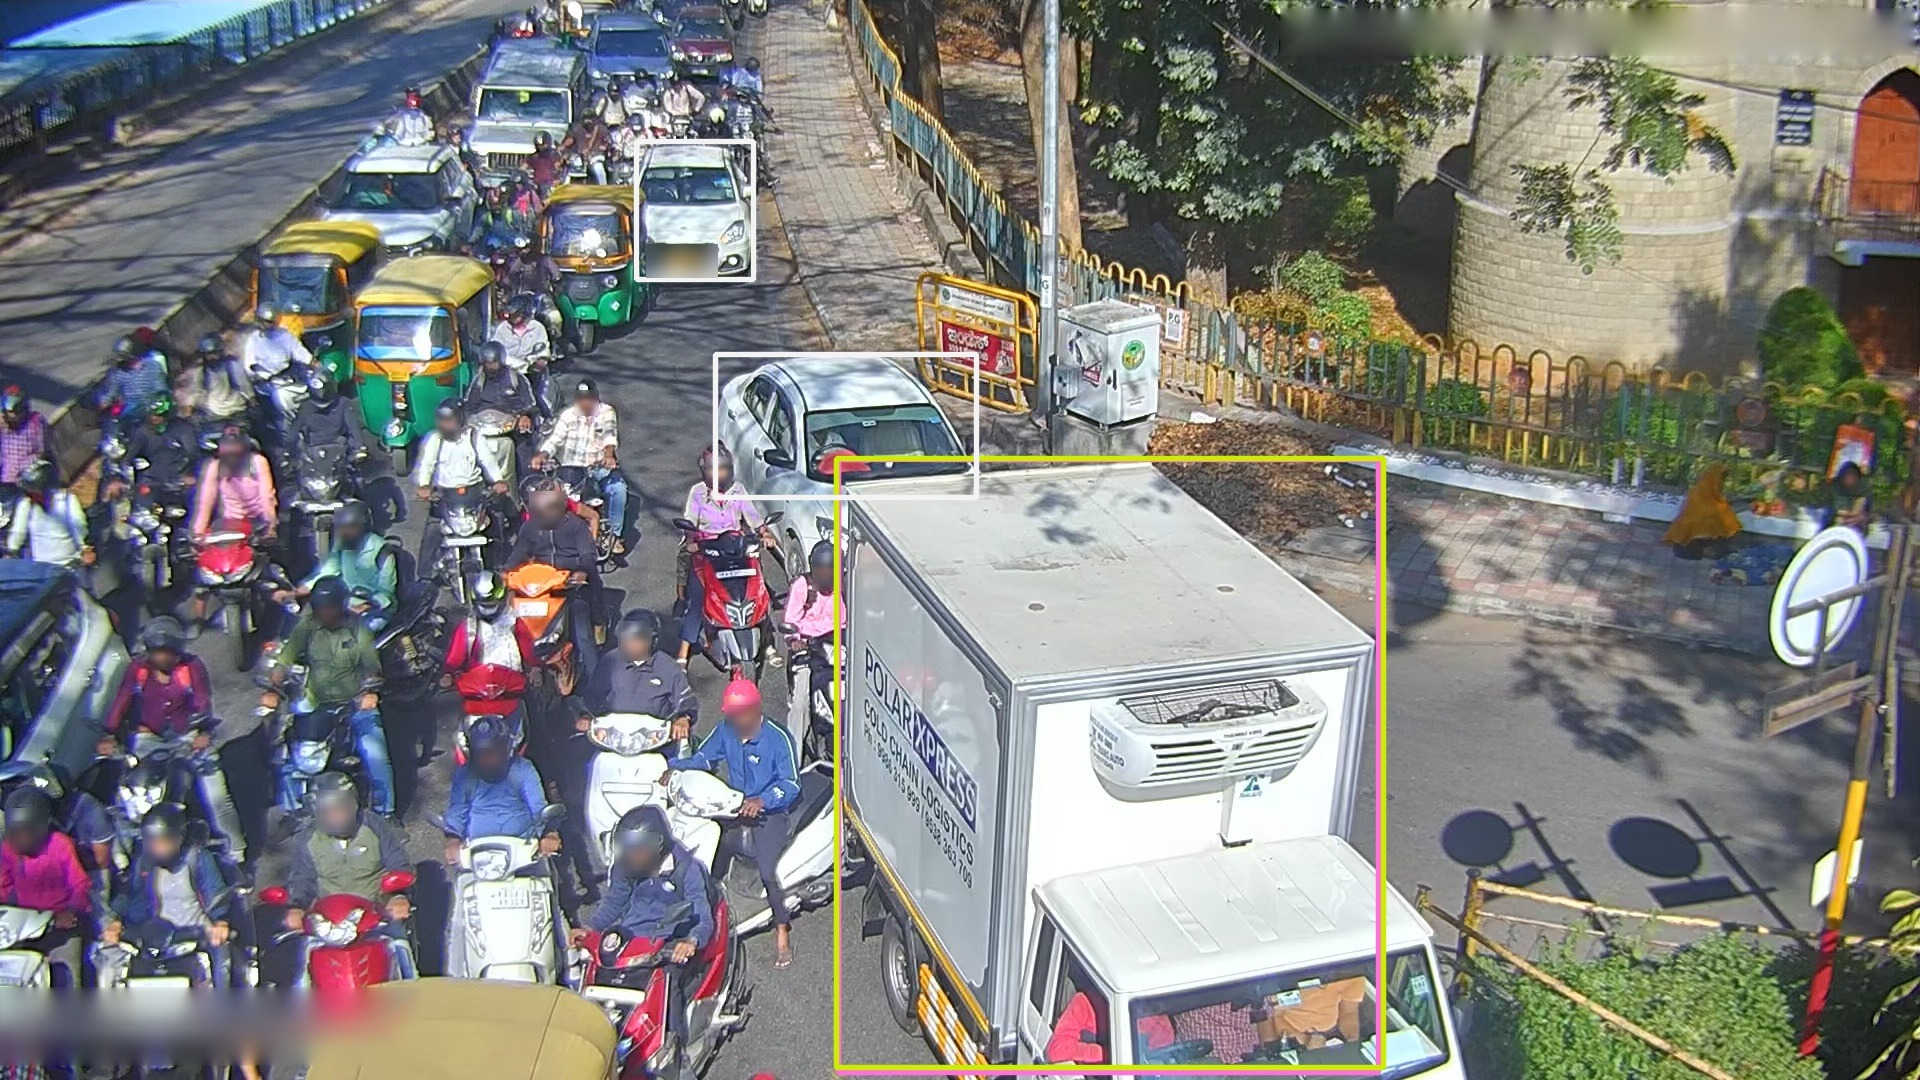
\includegraphics[width=\linewidth]{figures/scene1_base.jpg}
    \caption{YOLOv8n pré-entraîné (COCO) : 4 véhicules détectés.}
    \label{fig-demo-base}
  \end{subfigure}
  \hfill
  \begin{subfigure}{0.48\linewidth}
    \centering
    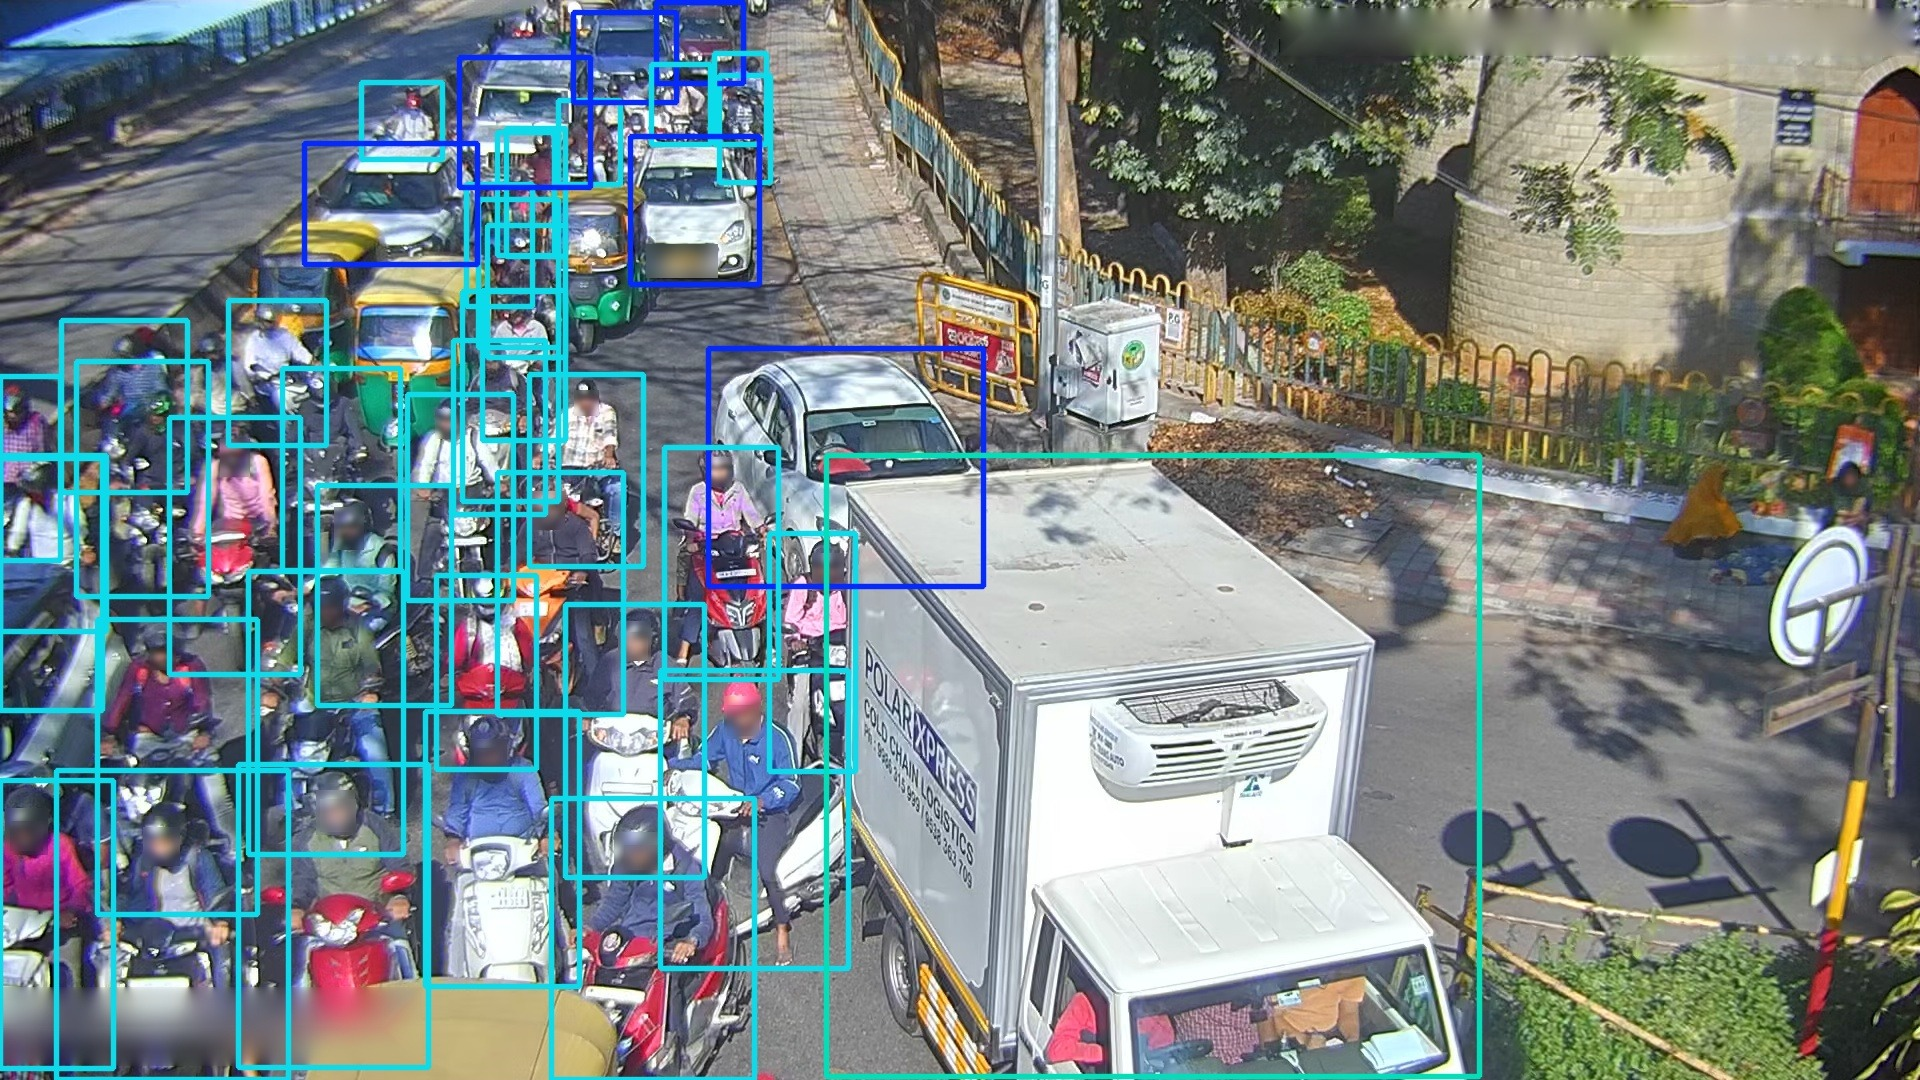
\includegraphics[width=\linewidth]{figures/scene1_finetune.jpg}
    \caption{YOLOv8n fine-tuné : 44 véhicules détectés.}
    \label{fig-demo-finetune}
  \end{subfigure}
  \caption{Détections des deux modèles sur une même scène
  d'embouteillage du jeu de test (image \texttt{val\_000556}, seuil de
  confiance $0{,}25$). Les visages sont floutés à la source dans BMD-45 ;
  la seule plaque d'immatriculation partiellement lisible a été floutée
  par nos soins.}
  \label{fig-demo}
\end{figure}

\begin{figure}[tb]
  \centering
  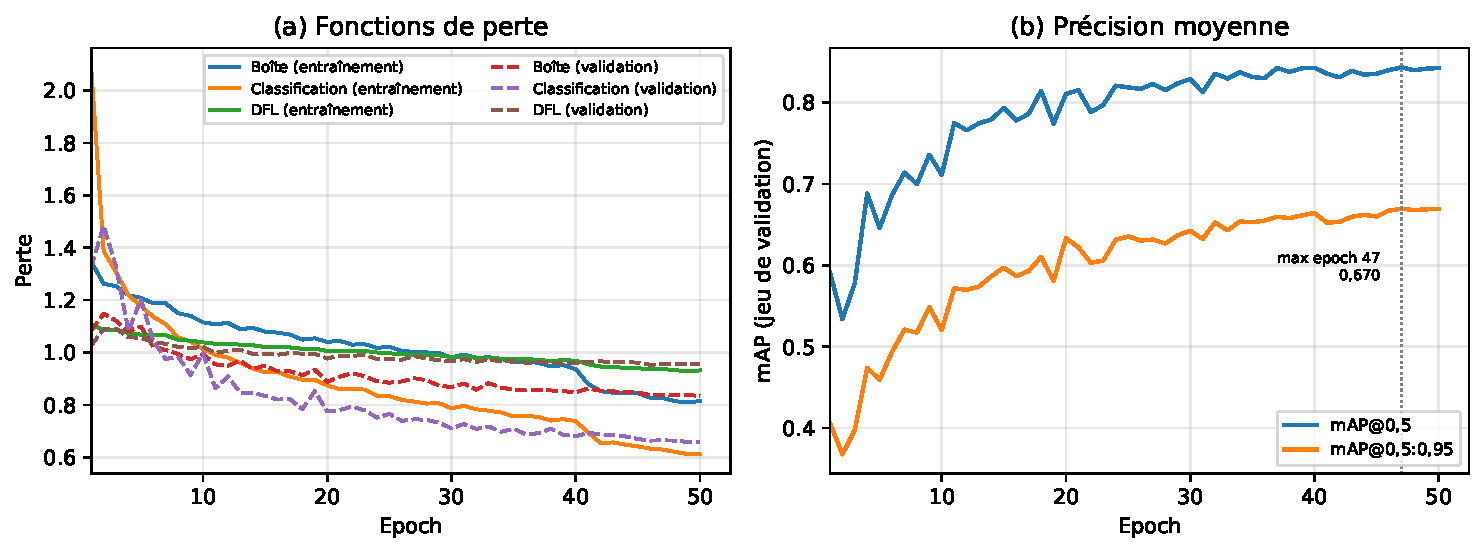
\includegraphics[width=\linewidth]{figures/courbes_entrainement.pdf}
  \caption{Courbes d'entraînement du fine-tuning : fonctions de perte
  (boîte, classification, DFL) et mAP@0,5 et mAP@0,5:0,95 sur le jeu de
  validation, au fil des 50 epochs. Les pertes d'entraînement sont en
  trait plein, celles de validation en pointillés. La ligne verticale
  marque l'epoch 47, où la mAP@0,5:0,95 de validation atteint son
  maximum.}
  \label{fig-courbes}
\end{figure}

\subsection{Dynamique d'entraînement}\label{sec-dynamique}

Les courbes de la \cref{fig-courbes} apportent trois informations que les
métriques finales seules ne donnent pas.

\paragraph{Une convergence rapide puis un plateau.}
La mAP@0,5:0,95 sur le jeu de validation passe de $0{,}406$ après la
première epoch à $0{,}669$ à la cinquantième, avec un maximum de
$0{,}670$ atteint à l'epoch 47. Elle franchit dès l'epoch 29 le seuil de
$95\,\%$ de sa valeur finale : les vingt et une dernières epochs
n'apportent que les $5\,\%$ restants. Le décrochage visible à l'epoch 2,
où la mAP@0,5 recule de $0{,}591$ à $0{,}534$, correspond à la montée en
puissance du taux d'apprentissage pendant la phase d'échauffement, et se
résorbe dès l'epoch 4. L'essentiel de l'adaptation au domaine se joue
donc dans le premier tiers de l'entraînement, ce qui est cohérent avec
l'idée que le fine-tuning réutilise des représentations déjà formées
plutôt qu'il n'en apprend de nouvelles.

\paragraph{Aucun surapprentissage à 50 epochs.}
Les trois pertes d'entraînement décroissent de façon monotone
($1{,}347 \rightarrow 0{,}814$ pour la boîte, $2{,}089 \rightarrow
0{,}611$ pour la classification, $1{,}107 \rightarrow 0{,}932$ pour la
DFL). Surtout, les pertes de validation atteignent leur minimum en toute
fin d'entraînement : epoch 50 pour la perte de boîte, 49 pour la
classification, 46 pour la DFL. L'écart entre pertes d'entraînement et
de validation ne se creuse à aucun moment, et l'arrêt anticipé
(\emph{patience} de 15 epochs, \cref{sec-entrainement}) n'a jamais été
déclenché. Le modèle n'avait donc pas commencé à surapprendre lorsque
l'entraînement s'est arrêté.

\paragraph{Le budget de calcul, et non la convergence, a fixé l'arrêt.}
Les deux observations précédentes se combinent en une conclusion
méthodologique : les 50 epochs constituent une borne que nous avons
imposée, pas un point d'arrêt que les données auraient dicté. Les
métriques rapportées au \cref{tab-comparaison} sont donc à lire comme un
plancher, et non comme le plafond de ce que cette architecture peut
atteindre sur ce jeu. L'entraînement complet a demandé $54{,}9$ minutes
sur GPU T4, ce qui laisse une marge confortable pour prolonger
l'expérience dans le cadre gratuit de Google Colab.

\section{Discussion}\label{sec-discussion}

\subsection{Le verrou visé est bien celui qui est levé}

La lecture centrale du \cref{tab-comparaison} est le gradient des gains
selon la taille des objets : $+469{,}4\,\%$ de rappel pour les objets
petits, $+135{,}6\,\%$ pour les moyens, $+20{,}2\,\%$ pour les grands.
L'amélioration est d'autant plus forte que l'objet est petit, c'est-à-dire
exactement là où le modèle générique échouait : le modèle pré-entraîné ne
retrouvait qu'un objet petit sur huit ($0{,}122$), le modèle fine-tuné en
retrouve plus des deux tiers ($0{,}694$). La réponse à la question de
recherche est donc positive, et elle l'est de manière ciblée : le
fine-tuning sur du trafic urbain dense n'améliore pas seulement les
métriques globales, il lève spécifiquement le verrou des véhicules
éloignés, de petite taille ou masqués qui motivait ce travail. Les
augmentations orientées petits objets (\emph{mosaic}, \emph{scale},
\cref{sec-entrainement}) et la densité du jeu d'entraînement
($8{,}5$ véhicules par image en moyenne) sont les explications les plus
plausibles de ce ciblage, sans que notre protocole permette d'isoler la
contribution de chacune ; une étude d'ablation serait nécessaire.

\subsection{Cohérence avec l'écart de domaine rapporté par BMD-45}

Notre passage de $0{,}296$ à $0{,}644$ de mAP@0,5:0,95, soit un facteur
$2{,}2$, est cohérent avec l'écart de domaine rapporté par les auteurs de
BMD-45~\cite{sharma2026bmd45} : des détecteurs entraînés sur
UA-DETRAC~\cite{wen2020uadetrac} atteignent $33{,}6\,\%$ de mAP@0,5:0,95
sur leur jeu, contre $83{,}8\,\%$ pour des modèles entraînés en domaine,
soit un facteur $2{,}5$. Nous retrouvons cet ordre de grandeur avec un
modèle nano et $6{,}7\,\%$ des images du jeu complet : l'essentiel de
l'écart entre un détecteur générique et un détecteur adapté semble donc
se combler dès un fine-tuning modeste, ce qui est une information
directement utile pour un déploiement à budget contraint.

\subsection{Ce que le fine-tuning ne résout pas}

Le rappel des objets petits plafonne à $0{,}694$ : 246 des 804 objets
petits du jeu de test restent non détectés. Une partie de ce résidu
relève d'une limite informationnelle et non d'un défaut de l'approche :
sous un certain nombre de pixels, l'information nécessaire à la détection
n'existe simplement plus dans l'image, et aucun modèle, quelle que soit
sa taille, ne peut la reconstituer. Ce plafond suggère que les marges de
progression restantes sont à chercher du côté de la résolution d'entrée,
de l'inférence par tuiles ou du placement des caméras, plutôt que du seul
entraînement.

Le gain de débit ($+16{,}2\,\%$, de $37{,}2$ à $43{,}2$ FPS) doit être
interprété avec prudence : l'architecture étant identique, il ne peut
provenir du réseau lui-même. L'hypothèse la plus plausible est un
post-traitement (suppression des non-maxima) allégé par la réduction de
80 à 4 classes, à quoi s'ajoute la variabilité de mesure inhérente à un
environnement partagé comme Google Colab. Nous n'avons pas conçu
d'expérience pour départager ces deux effets.

\subsection{Limites}

\paragraph{Domaine indien, contexte béninois.}
Il n'existe à ce jour aucun jeu de données public de vision par
ordinateur spécifique au Bénin. Nous avons donc travaillé sur du trafic
dense indien, structurellement comparable au trafic béninois sur trois
points : caméras CCTV fixes, forte densité, dominance des deux-roues
($56\,\%$ des instances, à rapprocher des zémidjans). Nos résultats
établissent que l'adaptation à un domaine de trafic dense de ce type est
possible et fortement bénéfique ; ils ne démontrent pas que le modèle
obtenu est adapté au trafic béninois lui-même. La constitution d'un jeu
de données local reste le préalable à toute conclusion de ce type.

\paragraph{Échelle des expériences.}
Le sous-ensemble utilisé représente 3\,000 images sur les 45\,000
disponibles, le modèle est la déclinaison nano, et l'entraînement est
limité à 50 epochs : ces choix, imposés par le temps machine disponible,
bornent la portée des chiffres absolus rapportés, même si la comparaison
relative entre les deux modèles reste valide puisqu'ils sont évalués dans
des conditions identiques.

\paragraph{Classes minoritaires.}
Les bus (189 instances) et camions (240 instances) sont minoritaires
dans le jeu de test : les métriques qui les concernent sont
mécaniquement moins stables que celles des voitures (742) et motos
(1\,380), et nous ne rapportons pas de métriques par classe pour cette
raison.

\paragraph{Contamination potentielle entre splits.}
Nos splits sont dérivés de façon déterministe, mais BMD-45 étant
constitué d'images de caméras fixes, des images quasi identiques
(même caméra, instants proches) peuvent se retrouver de part et d'autre
de la séparation train/test, un risque de contamination connu dans les
jeux publics qui tendrait à flatter les métriques absolues des deux
modèles sans invalider leur comparaison.

\paragraph{Protection des données personnelles.}
Les plaques d'immatriculation et les visages sont des données à
caractère personnel. Tout déploiement réel d'un système de
vidéoprotection au Bénin suppose un cadre juridique conforme au code du
numérique~\cite{benin2017code} et le contrôle de l'Autorité de
protection des données personnelles (APDP). Le présent travail, mené sur
un jeu de données public diffusé sous licence CC~BY~4.0, n'implique
aucune collecte de données.

\section{Conclusion}\label{sec-conclusion}

Nous avons montré qu'un fine-tuning modeste (3\,000 images, modèle
nano, 50 epochs sur un GPU T4) suffit à transformer un détecteur
générique en un détecteur adapté au trafic urbain dense, et que le gain
se concentre là où il était attendu : le rappel des véhicules de moins
de $32 \times 32$ pixels passe de $0{,}122$ à $0{,}694$
($+469{,}4\,\%$), tandis que la mAP@0,5 progresse de $0{,}438$ à
$0{,}825$ ($+88{,}4\,\%$), à débit d'inférence au moins égal. La valeur
du travail tient autant au protocole qu'aux chiffres : classes alignées
sur COCO et réindexées pour une comparaison équitable, rappel ventilé
par taille avec aires normalisées à la résolution d'entrée, jeu de test
isolé et dérivé de façon déterministe.

Trois prolongements se dégagent, par ordre de priorité. D'abord, la
constitution d'un jeu de données annoté de trafic béninois, préalable
indispensable pour transformer un résultat obtenu sur un domaine
comparable en un résultat établi sur le domaine cible, et dont ce
travail fournit le protocole d'évaluation clef en main. Ensuite, le
passage à l'échelle : entraîner sur les 45\,000 images de BMD-45 et sur
des déclinaisons plus grandes de YOLOv8 (s, m), pour mesurer ce que le
plafond observé sur les petits objets doit au modèle et ce qu'il doit à
la limite informationnelle. Enfin, la poursuite du pipeline de
vidéo-verbalisation (suivi multi-objets puis lecture de plaques), dont
la détection fiabilisée par ce travail constitue le socle.


\bibliographystyle{plain}
\bibliography{references}

\end{document}
